\documentclass[12pt]{article}
\usepackage{caption}

% Esto es para poder escribir acentos directamente:
\usepackage[utf8]{inputenc}
\usepackage[T1]{fontenc}

\usepackage{float}
\usepackage{enumerate} %-->

\usepackage[nottoc]{tocbibind}%-->

% Esto es para que el LaTeX sepa que el texto está en español españolao:
\usepackage[spanish]{babel}
\selectlanguage{spanish}%-->

\usepackage{titlesec}
\usepackage{titling}
\usepackage{xcolor}
\usepackage{hyperref}%compilar 2 veces
\usepackage{geometry}
\usepackage{listings}
\usepackage{pdfpages}
\usepackage{subfig}%figuras una alado de otraa


%% Paquetes de la AMS
\usepackage{amsmath, amsthm, amsfonts}%--->

%% Para añadir archivos con extensión pdf, jpg, png or tif
\usepackage{graphicx}%-->
\usepackage[colorinlistoftodos]{todonotes}%-->
%\usepackage[colorlinks=true, allcolors=blue]%{hyperref}%--->





\definecolor{commentsColor}{rgb}{0.13, 0.55, 0.13}
\definecolor{keywordsColor}{rgb}{0.000000, 0.000000, 0.635294}
\definecolor{stringColor}{rgb}{0.558215, 0.000000, 0.135316}
\definecolor{numerolineas}{rgb}{0.41,0.41,0.41}

\usepackage{verbatim}%coemntario begin%{} end

\usepackage{fancyhdr}%activar para usar encabezados esttilos funcy

%al final imprimir si solo utilizamos un printbibliografi  aqui el archivo bib
\usepackage[ backend=biber,style=apa]{biblatex}
\addbibresource{referencias.bib}%ojo con la ubicacion del bib y compilar con bibtex 

%\usepackage[top=1.5cm,bottom=1.0cm,left=1.25cm,right=1.25cm]%{geometry}%para todos las paginas




\providecommand{\keywords}[1]
{
  \small	
  \textbf{\textit{Keywords---}} #1
}

%% Primeroo escribimos el título
\title{Memoria Cache ,Bucles Anidados }
\author{Angel Andres Bejar Merma\\
  \small Universidad Nacional de San Agustin\\
  \small abejar@unsa.com\\
  \small Ciudad de Arequipa
  %\date{\today} 
}




\usepackage{listings}
\usepackage{xcolor}

\definecolor{codegreen}{rgb}{0,0.6,0}
\definecolor{codegray}{rgb}{0.5,0.5,0.5}
\definecolor{codepurple}{rgb}{0.58,0,0.82}
\definecolor{backcolour}{rgb}{0.95,0.95,0.92}

\lstdefinestyle{mystyle}{
    backgroundcolor=\color{backcolour},   
    commentstyle=\color{codegreen},
    keywordstyle=\color{magenta},
    numberstyle=\tiny\color{codegray},
    stringstyle=\color{codepurple},
    basicstyle=\ttfamily\footnotesize,
    breakatwhitespace=false,         
    breaklines=true,                 
    captionpos=b,                    
    keepspaces=true,                 
    numbers=left,                    
    numbersep=5pt,                  
    showspaces=false,                
    showstringspaces=false,
    showtabs=false,                  
    tabsize=2
}

\lstset{style=mystyle}
 




\begin{document}
%\newgeometry%{bottom=2.5cm,top=2.6cm,left=2.5cm,right=2.5cm}
%\restoregeometry
%\includepdf{9}

%
%paraa el report 


\maketitle

%% Aquí podemos añadir un resumen del trabajo (o del artículo en su caso) 
\begin{abstract}
    Se implementara y analizara el codigo de  bucles anidados  For ademas de comprender la función de  la memoria cache.
    \end{abstract}
    
    \keywords{Computación paralela, bucles, memoria, caché}%\begin{abstract}



%\end{abstract}

%\vspace{5mm} %espacio vertical usar en imagen



\section{Actividad}

Implementar y comparar los 2-bucles anidados FOR presentados en el cap. 2 del libro, pag 22.



\begin{figure}[H]%estricto
  \centering
  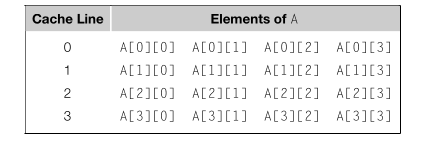
\includegraphics[width=15cm]{imagenes/Captura de pantalla de 2023-09-18 00-32-30.png}
 
  %\caption*{Prueba }
  
  \end{figure}
  

  En los siguientes funciones de codigo \ref{fig:algo}, esperaríamos que el primer par de bucles anidados tuviera un rendimiento mucho mejor que el segundo, ya que accede a los datos del array  de 2 bidimensional en bloques contiguos.




Entonces, por ejemplo, A[0][1] se almacena inmediatamente después de A[0][0] y A[1][0] se almacena inmediatamente después de A[0][3]. Supongamos que ninguno de los elementos de A está en el caché cuando cada par de bucles comienza a ejecutarse. Supongamos también que una línea de caché consta de cuatro elementos de A y A[0][0] es el primer elemento de una línea de caché.
Finalmente, supondremos que el caché está mapeado directamente y solo puede almacenar ocho elementos de A, o dos líneas de caché. (No nos preocuparemos por xey). Ambos pares de bucles intentan acceder primero a A[0][0]. Como no está en el caché, esto resultará en una pérdida de caché y el sistema leerá la línea que consta de la primera fila de A, A[0][0], A[0][1], A[0] [2], A[0][3], en el caché. Luego, el primer par de bucles accede a A[0][1], A[0][2], A[0][3], todos los cuales están en el caché, y el siguiente error en el primer par de bucles ocurre cuando el código accede a A[1][0].
Siguiendo de esta manera, vemos que el primer par de bucles dará como resultado un total de cuatro fallos cuando acceda a los elementos de A, uno para cada fila. Tenga en cuenta que dado que nuestro caché hipotético solo puede almacenar dos líneas u ocho elementos de A, cuando leemos el primer elemento de la fila dos y el primer elemento de la fila tres, una de las líneas que ya está en el caché tendrá que ser desalojada del caché, pero una vez que se expulsa una línea, el primer par de bucles no necesitará acceder a los elementos de esa línea nuevamente.
Después de leer la primera fila en el caché, el segundo par de bucles debe acceder a A[1][0], A[2][0], A[3][0], ninguno de los cuales está en el caché. Entonces los próximos tres accesos de A también resultarán en errores. Además, debido a que el caché es pequeño, las lecturas de A[2][0] y A[3][0] requerirán que se expulsen las líneas que ya están en el caché.

Dado que A[2][0] está almacenado en la línea de caché 2, leer su línea desalojará la línea 0, y leer A[3][0] desalojará la línea 1. Después de terminar el primer paso por el bucle externo, A continuación, deberá acceder a A[0][1], que fue desalojado con el resto de la primera fila. Entonces vemos que cada vez que leemos un elemento de A, fallaremos, y el segundo par de bucles resulta en 16 errores. Por lo tanto, esperaríamos que el primer par de bucles anidados fuera mucho más rápido que el segundo. De hecho, si ejecutamos el código en uno de nuestros sistemas con MAX = 1000, el primer par de bucles anidados es aproximadamente tres veces más rápido que el segundo par\cite{pacheco2011introduction}.






\newpage
\section{Análisis}



Se hizo 5 pruebas con memoria cache, de los cuales el segundo par de bucles anidado es mucha
mas lento en cuanto a tiempo de ejecución, esto se puede ver en la Fig \ref{fig:algo} ,

Esto debido a :

\begin{itemize}
  \item Primero :Teniendo en cuenta que la cache solo puede almacenar 2 líneas o 8 elementos de A y Amxn .
  Primer par de bucles; para acceder a el primer elemento de la matriz, esta resultará en una
 falla de caché, ya que esta no se encuentra en la caché, luego el sistema leerá toda la primera
 fila de A. Así  sucesivamente cometiendo m fallos.

 \item  Segundo : Después de leer la primera fila en la caché, este necesita acceder
 a A[1][0], A[2][0],...A[m][0], los cuales no se encuentran en caché por ende estos accesos
 resultarán en fallos, y debido a que la caché es muy pequeña las lecturas para acceder a las
 demás filas de A se requerirá que las líneas anteriores sean desalojadas. Esto se genera n
 Veces, por lo cual se tendrá m*n fallos\cite{cormen2022introduction}
 .
\end{itemize}

\section{Codigo}


El código \cite{pacheco2011introduction} implementado es el siguiente :

\lstinputlisting[language=c++]{algoritmo.cpp}




\section{Anexo}



\begin{figure}[H]%estricto
  \centering
  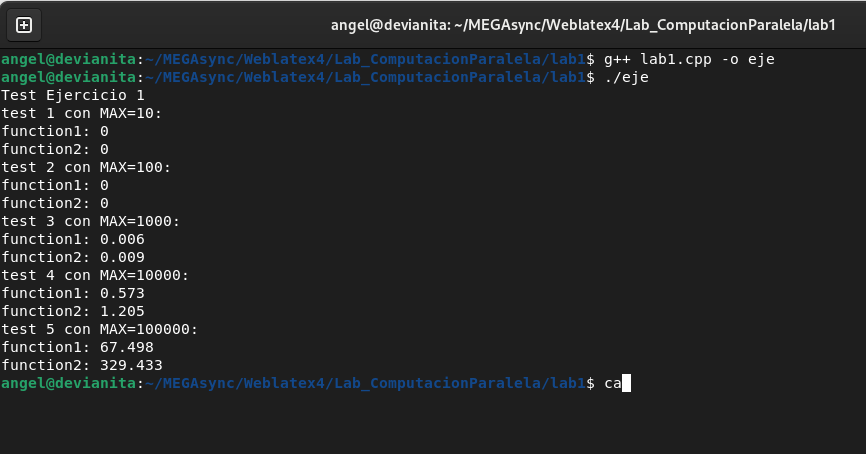
\includegraphics[width=15cm]{imagenes/Captura de pantalla de 2023-09-17 23-32-14.png}
  
  \caption{Prueba }
  \label{fig:algo}

\end{figure}







Repositorio: \url{https://github.com/ubuangel/Weblatex4/tree/main/Lab_ComputacionParalela/informes}

\vspace{20 mm}







\printbibliography

\end{document}

